This chapter contains the controller design for the refrigeration system model developed in \cref{sec:mod}. A simple pole-placement method controller will be made as an initial step to verify that the model is sufficient and to get a feel for the system before moving on to a more complex controller. An MPC controller is chosen due to its ability to handle constraints which is essential for handling the actuator limitations in a reefer system. Both the pole-placement and MPC controller will be benchmarked against the coupled PID controllers currently implemented at BITZER.


\subsection{State space controller - Pole placement}
The poles of a controllable state space system is the eigenvalues of the system matrix $(A)$. When the states of a state space system is fed back through a feedback gain $(K)$ the system matrix of the closed-loop system becomes:

\begin{equation} \label{eq:A_cl}
	A_{cl} = A-BK
\end{equation}

If \cref{fig:state_space_fb} is analyzed by looking at the how $\dot{x}$ is calculated from $x$ this becomes obvious. A controllable system has the appealing property of  pole placement. This means that in theory the poles of the system can be moved anywhere to achieve some specific behavior. Such a change could be to make the system faster by placing them further to the left in the complex plane.

\begin{figure}[h!]
	\centering
	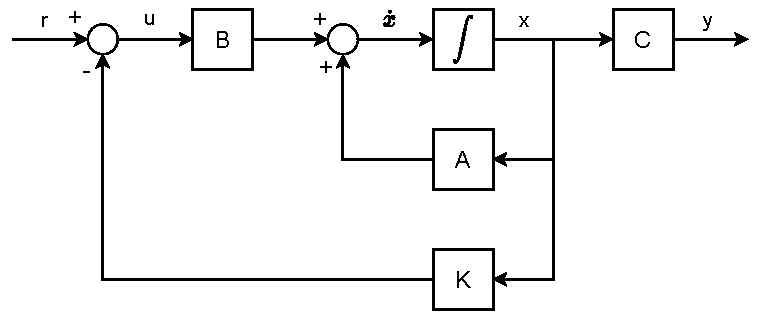
\includegraphics[width=0.60\textwidth]{Graphics/State_space_feedback.pdf}
	\caption{Generic state-space system with feedback}
	\label{fig:state_space_fb}
\end{figure}


% SIXO system pole placement algorithm
%For a \underline{SISO} system the poles can be placed by hand from the following algorithm:
%\begin{enumerate}
%	\item defining desired pole placements for all system poles and writing out the characteristic polynomial for these wanted system poles e.g.
%	$(s-p_1)(s-p_2) \cdots (s-p_n) = s^n + a_{cl_1} \cdot s^{n-1} + a_{cl_2} \cdot s^{n-2} \cdots a_{cl_n}$
%	\item calculating the eigenvalues of \cref{eq:A_cl} which yields the characteristic polynomial of the feedback system e.g.
%	$det(A_{sys}) = s^n + (a_{sys_1}-k_1) \cdot s^{n-1} + (a_{sys_2}-k_2) \cdot s^{n-2} \cdots (a_{sys_n}-k_n)$
%	\item setting the coefficients of the characteristic polynomial of the native system equal to the coefficients of the desired pole placement and solving for the entries in K e.g.
%	$ k_1 = a_{sys_1}-a_{cl_1}, k_2 = a_{sys_2}-a_{cl_2} \cdots k_n = a_{sys_n}-a_{cl_n} $
%	 This yields the $ K = [k_1, k_2 \cdots k_n]^T $ which places the poles at the desired location.
%	\item x is fed back through K to the input yielding \cref{eq:A_cl}.
%\end{enumerate}
%
%In Matlab the above algorithm can be performed by the simple function \textit{Place(A, B, poles)} where "A" is the system matrix, "B" the input matrix and "poles" an array of the desired poles. The \textit{place()} works for both SISO and MIMO systems.

In Matlab pole placement can be performed by the \textit{Place(A, B, poles)} function where "A" is the system matrix, "B" the input matrix and "poles" an array of the desired poles. The \textit{place()} function works for both SISO and MIMO systems.






\subsection{LMI / MPC controller}
Model Predictive Control (MPC) is, like the Linear Quadratic Regulator (LQR), an optimal control algorithm with respect to some cost function. It is optimal with regards to the current sample but in contrast to LQR it also takes future samples into account. It relies on a dynamic model of the controlled process and is able to consider various types of constraints.\\

At every time sample the MPC controller
\begin{enumerate}
	\item optimizes over \textit{prediction horizon} $(H_p)$
	\item calculates a predictive optimal control trajectory
	\item applies the first sample in the predicted control trajectory to the process
\end{enumerate}

\medskip

Consider the discrete-time system in \cref{eq:mpc_discrete_sys}. While $y(k)$ represents the measured outputs, $z(k)$ represents the controlled non-measured outputs. It is possible that $y(k) = z(k)$ in this case all controlled outputs are measured.

\begin{equation} \label{eq:mpc_discrete_sys}
	\begin{split}
		x(k+1) 	& = Ax(k) + Bu(k) \\
		y(k) 	& = C_yx(k) \\
		z(k) 	& = C_zx(k)
	\end{split}
\end{equation}

For such a system the MPC controller optimizes with respect to the quadratic cost function in \cref{eq:mpc_cost_fcn}. The first part of the cost function seeks to minimize the deviation of the controlled states $(\hat{z})$ from the reference trajectory $(r)$ over the prediction horizon where $Q(i)$ are the weights applied at each predicted sample. The second part insures integral action by minimizing change in control input $(\Delta \hat{u})$ (control moves) over the \textit{control horizon} $(H_u)$ where $R(i)$ are the weights applied to each control move into the future.

\begin{equation} \label{eq:mpc_cost_fcn}
	V(k) = \sum_{i=H_w}^{H_p}||\hat{z}(k+i|k) - r(k+i|k)||^2_{Q(i)} + \sum_{i=0}^{H_u-1}||\Delta \hat{u}(k+i|k)||^2_{R(i)}
\end{equation}

where

\begin{center}
	\begin{tabular}{l r l }
		                   & $||x||_M$               & $= \sqrt{\left(w^TMw\right)}$                    \\
		prediction horizon & $H_p$                   & $\ge$ $H_u$ control horizon           \\
		window horizon     & $H_p$                   & $\ge 1$                               \\
		weights            & $Q(i), R(i)$            & $\ge 0$ (positive semi-definite)      \\
		control move       & $\Delta \hat{u}(k+i|k)$ & $= \hat{u}(k+i|k) - \hat{u}(k+i-1|k)$
	\end{tabular}
\end{center}

$Q(i), Q(i), H_p, H_u, H_w$ are considered the MPC tuning parameters.\\

An important characteristic of MPC is the ability to include constraints. Constraints can be applied to \textit{actuator slew rate}, \textit{actuator range} and \textit{controlled variables}. These constraints need to be formulated in the correct manner as seen below:

\begin{itemize}
	\item Actuator slew rate:

	\begin{equation} \label{eq:mpc_const_sr}
		E \begin{bmatrix} \Delta U(k) \\ 1 \end{bmatrix} \le 0
	\end{equation}
	\begin{center} where \end{center}
	\begin{equation*}
		\Delta U(k) = [\Delta \hat{u}(k|k)^T \cdots \Delta \hat{u}(k+H_u-1|k)^T]^T
	\end{equation*}


	\item Actuator range:

	\begin{equation} \label{eq:mpc_const_ar}
		F \begin{bmatrix} U(k) \\ 1 \end{bmatrix} \le 0
	\end{equation}
	\begin{center} where \end{center}
	\begin{equation*}
		U(k) = [\hat{u}(k|k)^T \cdots \hat{u}(k+H_u-1|k)^T]^T
	\end{equation*}

	\item Controlled variable

	\begin{equation} \label{eq:mpc_const_cv}
		G \begin{bmatrix} Z(k) \\ 1 \end{bmatrix} \le 0
	\end{equation}
	\begin{center} where \end{center}
	\begin{equation*}
		Z(k) = [\hat{z}(k+H_w|k)^T \cdots \hat{z}(k+H_p|k)^T]^T
	\end{equation*}
\end{itemize}

\noindent with E, F and G having appropriate dimensions.
